
%!TEX TS-program = xelatex
%!TEX encoding = UTF-8 Unicode


%% document settings
\documentclass[12pt]{article}
%=====================================================================
%=========================== fonts ===========================

	\usepackage[leqno,tbtags]{amsmath}
	\usepackage{amssymb}
	\usepackage{euler}
	\usepackage{dutchcal}
	\usepackage{xunicode,xltxtra, polyglossia}
	\usepackage{fontspec} %(include if mathspec is not loaded)
	\defaultfontfeatures{Mapping=tex-text, Ligatures=TeX}
	\setromanfont[Mapping=tex-text, Numbers={Proportional}]{Times New Roman}
	\setsansfont[Scale=MatchLowercase,Mapping=tex-text]{Optima}
	\setmonofont[Scale=MatchLowercase]{Andale Mono}
	\newfontfamily\opt{Optima}
	\usepackage[dvipsnames]{xcolor}

%=====================================================================
%=========================== page geom + layout ===========================

	\usepackage[margin = 1in]{geometry}

	\usepackage{titlesec}
		\titleformat{\section}{\sffamily\Large\bfseries}{\thesection}{1em}{}
		\titleformat{\subsection}{\sffamily\large\bfseries}{\thesubsection}{1em}{}
		\titleformat{\subsubsection}{\sffamily\normalsize\bfseries}{\thesubsubsection}{1em}{}

	\usepackage{titling}
	\pretitle{\begin{center}\opt\Large\bfseries}  % Title font style
	\posttitle{\end{center}}

	\clubpenalty10000
	\widowpenalty10000

	\usepackage{multicol}


%=====================================================================
%=========================== text ===========================

	% punctuation
		\setdefaultlanguage[variant=american]{english}
		\usepackage{csquotes} % for quotation marks
		\DeclareRobustCommand\dash{%
			\unskip\nobreak\thinspace\textemdash\thinspace\ignorespaces}

	% HYPHENATION RULES
		\RequirePackage{hyphenat}
		\hyphenation{
		  ana-phor ana-pho-ra ana-pho-ric
		  ana-ly-sis ana-ly-ses
		  %b
		  boo-le-an
		  mo-dal
		  nes-ted
		  spea-ker
		}

	% Formulas
		\newcommand{\transl}{\ensuremath{\rightsquigarrow}}
		\newcommand{\indef}{\reflectbox{$\varepsilon$}}
		% \def\co{\colon\thinspace}


%=====================================================================
%=========================== bib ===========================

	\usepackage[round]{natbib}
	\newcommand{\posscite}[1]{\citeauthor{#1}'s (\citeyear{#1})}


%=====================================================================
%=========================== ling packages ===========================
	\usepackage{stmaryrd}
	\usepackage{linguex}

%====================================================================
%=========================== links, references =======================
	\usepackage[colorlinks, hyperfootnotes=false]{hyperref}
	\hypersetup{allcolors=MidnightBlue} 
	\usepackage{cleveref} %better references
	% linguex options
		\renewcommand{\firstrefdash}{}%
		\AtBeginDocument{\settowidth{\Exlabelwidth}{(110)}}
	% more linguex options for referencing select examples without parentheses
	  \newif\ifparens\parensfalse
	  \makeatletter
	  \renewcommand{\theExNo}{\protect\theExLBr\arabic{ExNo}\protect\theExRBr}
	  \renewcommand{\theSubExNo}{%
	    \hbox{\if@noftnote\protect\theExLBr\Exarabic{ExNo}\firstrefdash
	        \Exalph{SubExNo}\protect\theExRBr
	      \else
	        \protect\theFnExLBr\Exroman{FnExNo}\firstrefdash%
	        \Exalph{SubExNo}\protect\theFnExRBr
	      \fi}}

	  \renewcommand{\theSubSubExNo}{%
	    \hbox{\if@noftnote\protect\theExLBr%
	            \Exarabic{ExNo}\firstrefdash\Exalph{SubExNo}\secondrefdash
	               \Exroman{SubSubExNo}\protect\theExRBr%
	      \else\protect\theFnExLBr\Exroman{FnExNo}\firstrefdash
	                \Exalph{SubExNo}\secondrefdash\Exarabic{SubSubExNo}\protect\theFnExRBr\fi}}%
	  \makeatother
	  \renewcommand\theExLBr{\ifparens\else(\fi}
	  \renewcommand\theExRBr{\ifparens\else)\fi}
	  \newcommand\pref[1]{{\parenstrue\ref{#1}}}




%=====================================================================
%=========================== figures, tables =========================
	% \RequirePackage{tikz} % for drawing diagrams
	% \tikzstyle{opaque}=[fill=gray,fill opacity=.1] % tikz option
	% \RequirePackage{pbox} % for alignment in diagrams
	\RequirePackage{booktabs} % for prettier tables
	% \usepackage{easybmat}
	\usepackage{tikz}
	\usepackage{venndiagram}
	\usepackage{subfig}




% JT also loaded these packages
\usepackage{enumitem}
\usepackage{caption}
%\usepackage{subcaption}

\title{What is at-issueness? An experimental comparison of diagnostics}
\author{\normalsize Lisa Hofmann, Conglei Xu, Judith Tonhauser}
\date{\small\today}


\begin{document}
\maketitle
\begin{abstract}
  At-issueness is a key concept in theoretical semantics/pragmatics, but there is no consensus about how it is defined or diagnosed (e.g., \citealt{tonhauser_diagnosing_2012,tonhauser_how_2018,koev_notions_2018}). We present experimental data investigating whether four widely used diagnostics for at-issueness yield consistent results. Our findings reveal significant differences across diagnostics, indicating they are not interchangeable. Since the diagnostics target distinct theoretical conceptions of at-issueness, these differences offer insight into their comparability.
\end{abstract}
\setcounter{tocdepth}{2}
\tableofcontents
\pagebreak


\section{Introduction}
\label{sec:1_introduction}
  Although at-issueness is a central concepts in semantics and pragmatics, the literature has not come up with a unified notion of at-issueness. Rather, the literature comes with various theoretical notions (\citealt{koev_notions_2018,tonhauser_how_2018}) and empirical reflexes used to diagnose them (e.g., \citealt{tonhauser_diagnosing_2012}). Identifying distinct notions of at-issueness used in the literature, \citealt{koev_notions_2018} raised the question \emph{Do the diagnostics that fall out from the different theories make comparable predictions about the same type of content?} (p. 10). Based on impressionistic off-line judgments there are at least some types of contents for which the diagnostics yield different results, suggesting that they may diagnose related, but distinct notions of at-issueness. However, since the previous literature does not not paint an empirically clear picture, we experimentally compared four commonly used diagnostics for at\hyp issueness.

  The four diagnostics we tested are illustrated in (\pref{qud}--\pref{yesbut}) for sentence-medial non-restrictive relative clauses (NRRCs), which are usually taken to contribute non-at-issue content.  As appositive content is generally taken to be not-at-issue, participants are expected to: Give low naturalness ratings under the QUD diagnostic \ref{qud} and the direct dissent diagnostic \ref{dd}, not interpret the speaker to be asking about the content under the `asking-whether' diagnostic in \ref{aw}, will choose one of the %indirect denials with 
    \emph{yes}-responses under the `yes, but' diagnostic in \ref{yesbut}.

    \ex. \label{qud}%
      QUD diagnostic (e.g., \citealt{tonhauser_diagnosing_2012,chen_presuppositions_2024})
      \a.[A:] \emph{What did Greg buy?}
      \b.[B:] \emph{Greg, who bought a new car, is envied by his neighbor.}
      \z.
      Question to participants: How well does B's response fit A's question?
    \z.

    \ex. \label{aw}%
      `asking whether' diagnostic (e.g., \citealt{tonhauser_how_2018,solstad_cataphoric_2024})\smallskip\\
        \emph{Is Greg, who bought a new car, envied by his neighbor?}\smallskip
    \\ Question to participants: Is the speaker asking whether Greg bought a new car?
    \z.

    \ex. \label{dd} Direct dissent diagnostic (e.g., \citealt{tonhauser_diagnosing_2012,syrett_experimental_2015})
      \a.[A:] \emph{Greg, who bought a new car, is envied by his neighbor.}
      \b.[B:]\emph{No, that's not true, he didn't buy a new car.}
      \z.
    Question to participants: How natural is B's rejection of A's utterance?
    \z.

    \ex. \label{yesbut}%
      `yes, but' diagnostic (e.g., \citealt{xue_correlation_2011,schwarz_cross-linguistic_2015})
      \a.[A:] \emph{Greg, who bought a new car, is envied by his neighbor.}
      \b.[B:] \emph{Yes, but he didn't buy a new car.} /
      \b.[] \emph{Yes, and he didn't buy a new car.} /
      \b.[] \emph{No, he didn't buy a new car.}
      \z.
      Task for participants: Choose the response that sounds best.
    \z.

    The diagnostics reflect different theoretical conceptions of at-issueness: The QUD diagnostic targets Q-at-issueness (\citealt{koev_notions_2018}), the `asking whether' diagnostic assumes that  (\citealt{tonhauser_how_2018}); and the direct dissent and `yes, but' diagnostics reflect P-at-issueness.
   

  \paragraph{Theoretical notions}
    \citealt{koev_notions_2018}
    \begin{itemize}
      \item  Q-at-issueness, where at-issue content addresses the QUD
      \item P-at-issueness, where at-issue content constitutes a proposal to update the common ground
      \item mention C-at-issueness, which is assumed to be a gerenalization of P-at-issueness, and further discussed later
    \end{itemize}

    \citealt{tonhauser_how_2018}
    \begin{itemize}
      \item at-issue content of interrogatives partitions the context set (related to both Q-at-issueness, and P-at-issueness)
    \end{itemize}

  \paragraph{Diagnostics and theory.} (integrate into above discussion)
    

  \paragraph{Previous research.} (what do they tell us about question from koev)
    Prior research has identified disagreements, potentially arising from  diagnostic differences:

    Based on , \citealt{koev_notions_2018} suggests that medial appositives can be Q-at-issue, but not P-at-issue. While \citealt{syrett_experimental_2015} found that sentence-medial appositives are less at-issue than sentence-final ones using the direct dissent test, \citealt{drozdov_projection_2024} found no difference with the `asking whether' diagnostic.

    To investigate how consistent the diagnostics are, we conducted four experiments measuring the at-issueness of the same contents across diagnostics.

  \paragraph{Questions} % (fold)
    \begin{enumerate}
      \item Do different diagnostics of at-issueness yield the same results when testing the same stimuli?
      \item Do the results support the notion that different theoretical conceptions of at-issueness are distinct?
      % \item Do the results support the notion that different diagnostics under the same theoretical conceptions modulate the at-issueness of contents?
    \end{enumerate}

\section{Experiments}

To compare the results of at-issueness diagnostics, we conducted four experiments that each measured at-issueness with a different diagnostic, namely the QUD diagnostic (Exp.~1), the `asking whether' diagnostic (Exp.~2), the direct dissent diagnostic (Exp.~3) and the `yes, but' diagnostic (Exp.~4). To be able to compare the results of the diagnostics, the same seven contents shown in \ref{stims} were investigated under the four diagnostics, namely the contents of sentence-medial and sentence-final NRRCs, as well as the contents of the clausal complements of \emph{know, discover, confess, confirm} and \emph{be right}. These seven contents were instantiated by the same items across the four experiments.
  
    \ex.\label{stims}
      \a.\label{stims.a} Content of sentence-medial NRRC \\
        \emph{Lucy, who broke the plate, apologised.} $\leadsto$ Lucy broke the plate
      \b.\label{stims.b} Content of sentence-final NRRC \\
      \emph{The police found Jack, who saw the murder.} $\leadsto$ Jack saw the murder
      \c.\label{stims.c} Content of the clausal complement of \emph{know} \\
      \emph{Ann knows that Raul cheated on his wife.} $\leadsto$ Raul cheated on his wife
       \d.\label{stims.d} Content of the clausal complement of \emph{discover} \\
      \emph{Mary discovered that Denny ate the last cupcake.} $\leadsto$ Denny ate the last cupcake
       \e.\label{stims.e} Content of the clausal complement of \emph{be right} \\
      \emph{Tom is right that Ann stole the money.} $\leadsto$ Ann stole the money
       \f.\label{stims.f} Content of the clausal complement of \emph{confirm} \\
      \emph{Harry confirmed that Greg bought a new car.} $\leadsto$ Greg bought a new car
       \z.\label{stims.g} Content of the clausal complement of \emph{confess} {\bf JT hates linguex. This is one of the reasons} \\
      \emph{Lucy confessed that Dustin lost his key.} $\leadsto$ Dustin lost his keys
    \z.
    
In each experiment, participants read the stimuli and gave ratings corresponding to the diagnostics.  


  \subsection{Methods}
  
\subsubsection{Participants}

For each of the four experiments, we recruited 80 participants on Prolific. These participants had registered on the platform as
monolingual native speakers of English who lived in the USA. They had at least 100 previous submissions
and an approval rate of at least 97\%.

Table \ref{t:recruited}...

\begin{table}[h!]
\centering
\begin{tabular}{l | c | r r r r r r}
            & recruited & ages & mean age & female & male & nonbinary & did not disclose \\ \hline
Exp.~1 & &  &  & &  & &  \\
Exp.~2 & &  &  & &  & &  \\
Exp.~3 &&  &  & &  & &  \\
Exp.~4 &&  &  & &  & &  \\
\hline
\end{tabular}

\caption{Information about the participants recruited in Exps.~1-4.}\label{t:recruited}
\end{table}
      
\subsubsection{Materials and procedure}

     Each content type was instantiated by one of seven items (e.g., `Greg bought a new car') and realized as either an assertion \ref{qud}, \ref{dd}, \ref{yesbut} or a polar question \ref{aw}. Participants responded for the seven target stimuli and two control stimuli, by adjusting a slider for (\pref{qud}--\pref{dd}), or by choosing a response in \ref{yesbut}.
     
\begin{figure}[h!]
\centering

\begin{subfigure}{.49\textwidth}
\centering
\fbox{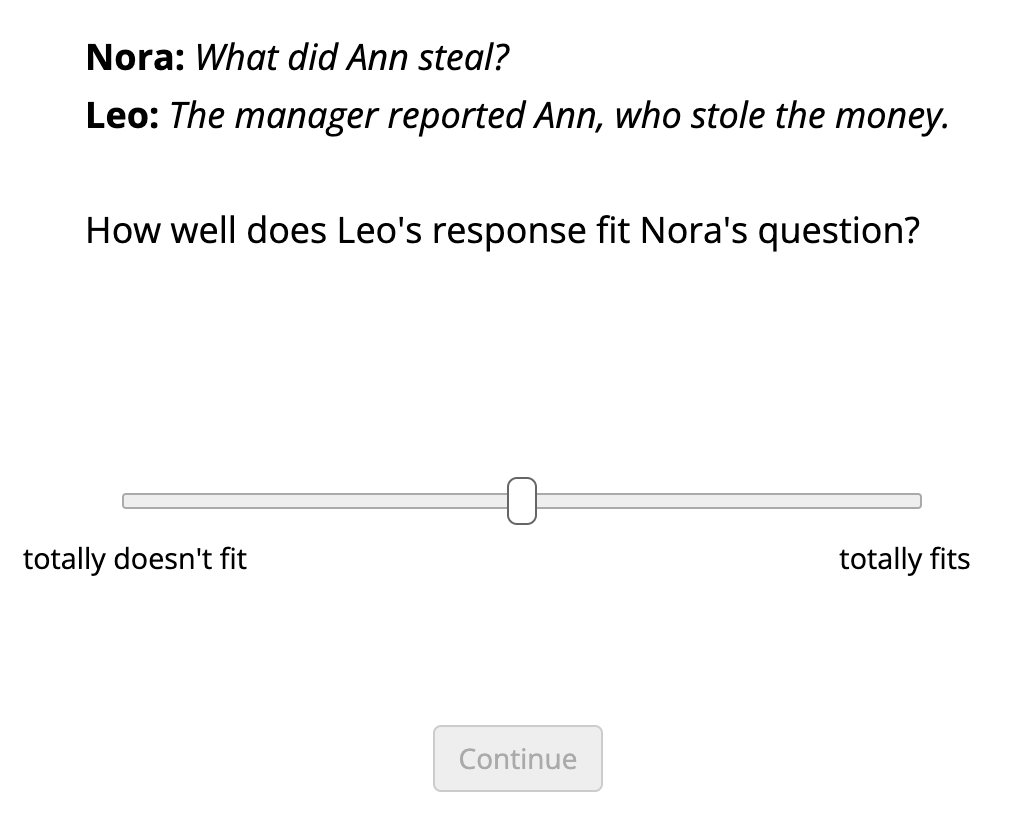
\includegraphics[width=1\textwidth]{figures/trialExp1}}
 \caption{Exp.~1: QUD diagnostic}
 \end{subfigure} 
 \begin{subfigure}{.49\textwidth}
\centering
\fbox{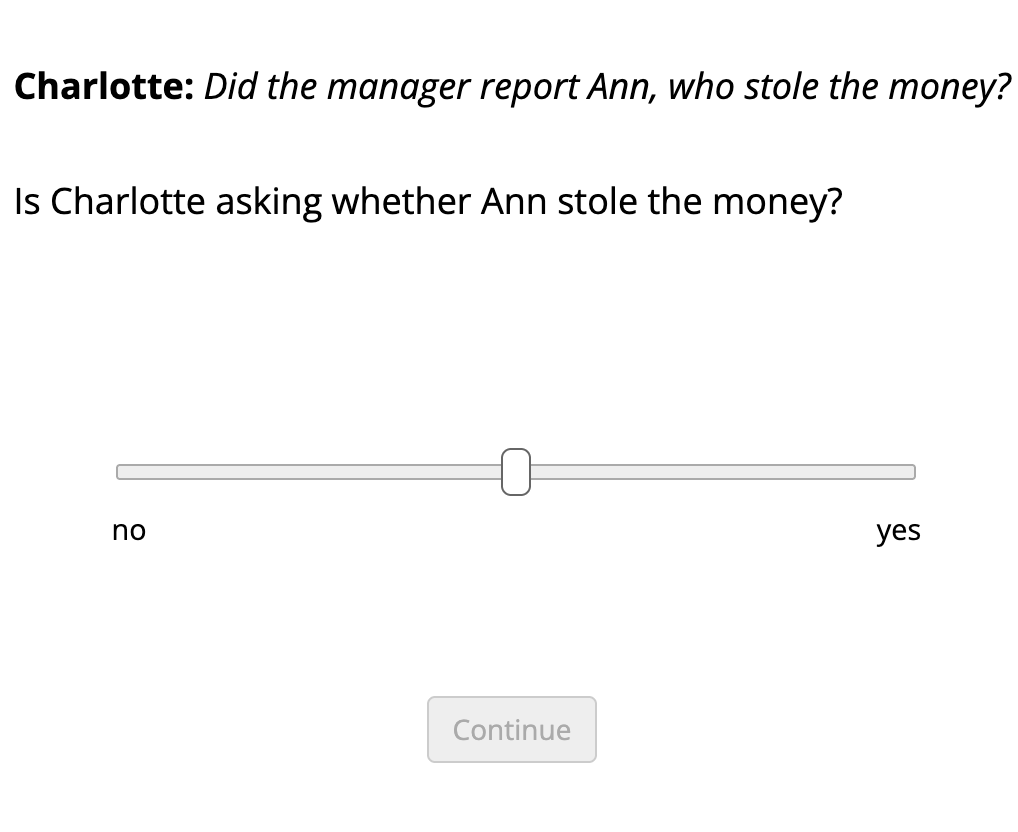
\includegraphics[width=1\textwidth]{figures/trialExp2}}
 \caption{Exp.~2: `asking whether' diagnostic}
 \end{subfigure}

\begin{subfigure}{.49\textwidth}
\centering
\fbox{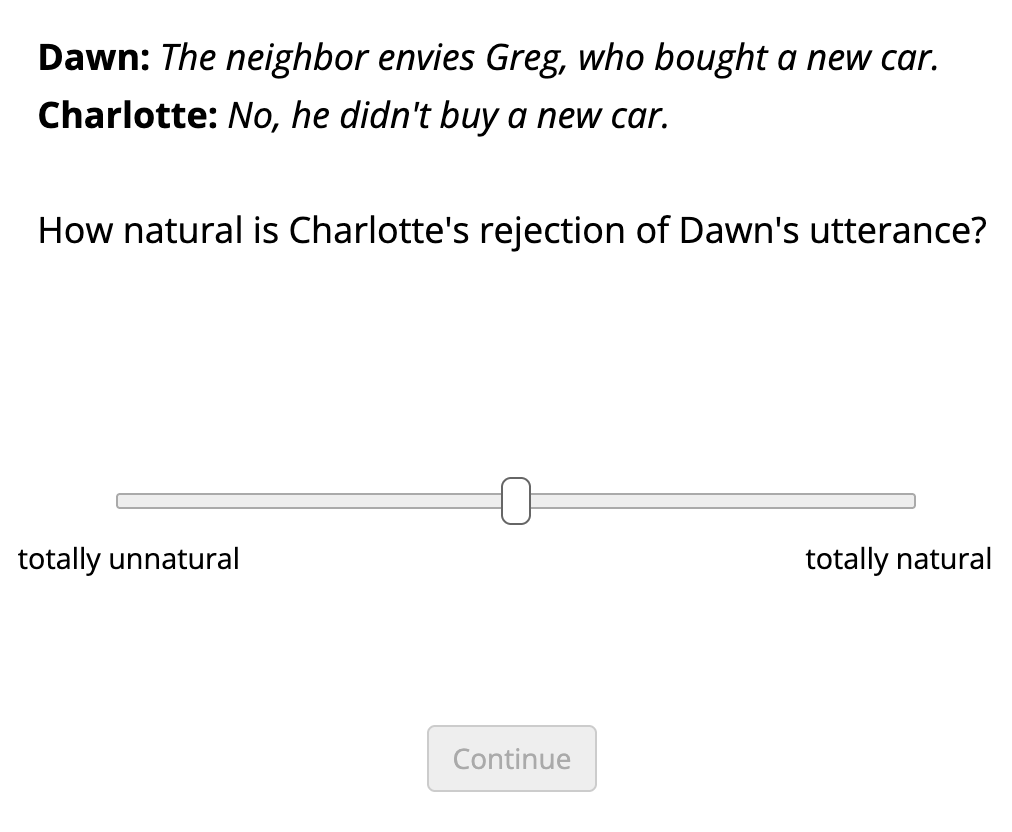
\includegraphics[width=1\textwidth]{figures/trialExp3}}
 \caption{Exp.~3: `direct dissent' diagnostic}
 \end{subfigure} 
 \begin{subfigure}{.49\textwidth}
\centering
\fbox{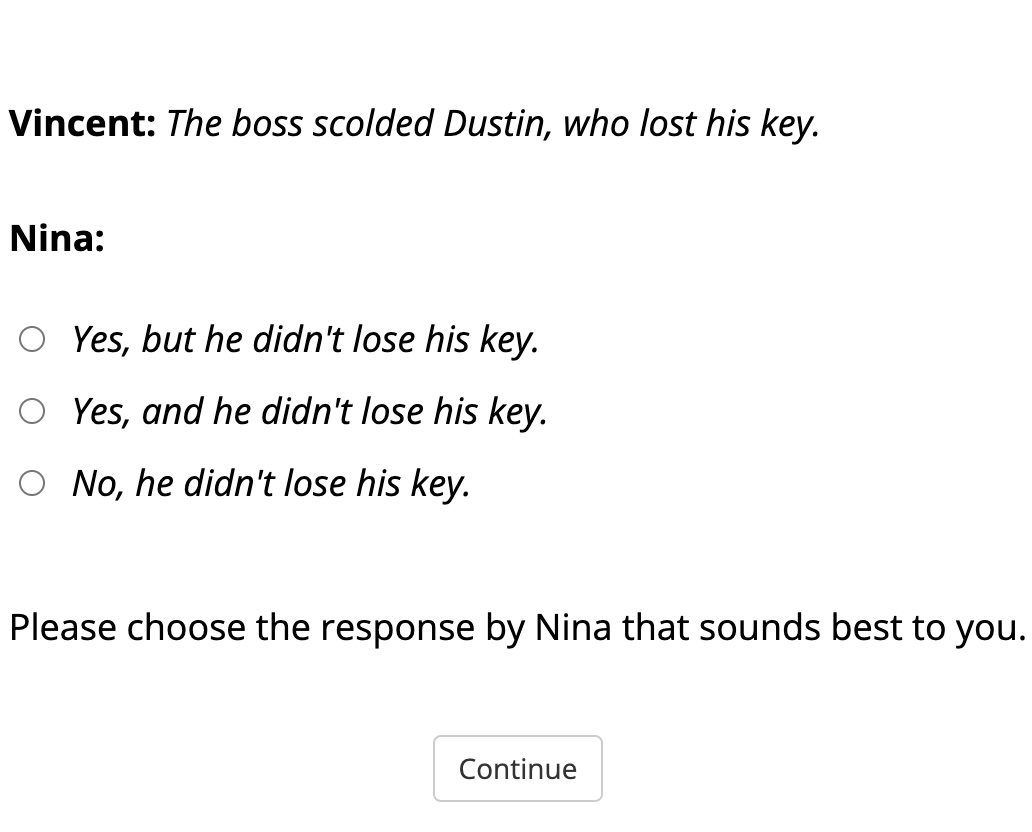
\includegraphics[width=1\textwidth]{figures/trialExp4}}
 \caption{Exp.~4: `yes, but' diagnostic}
 \end{subfigure}

\caption{Sample trials in (a) Exp.~1, (b) Exp.~2, (c) Exp.~3 and (d) Exp.~4.} \label{fig:trials}

\end{figure}


\subsubsection{Data exclusion}

We excluded the data of participants who did not self-identify as native speakers of
American English and of participants whose responses to the xxx was more than 2 sd away from the group mean WHAT ABOUT EXP 4?

Table \ref{t:excluded} identifies how many participants were excluded in each experiment, the properties of the remaining participants, and the number of data points that entered into the analyses.

\begin{table}[h!]
\centering
\begin{tabular}{l r | r r | r r r r r r | r}
             & & \multicolumn{2}{c}{exclusion criterion} & \multicolumn{6}{c}{remaining participants} & \\ 
            & recruited & language & fillers & ages & mean age & f & m & nb & dnd & data points \\ \hline
Exp.~1 &  &  &  &  &  &  & &  & & \\ 
Exp.~2 &  &  &  &  &  &  & &  & & \\ 
Exp.~3 &  &  &  &  &  &  & &  & & \\ 
Exp.~4 &  &  &  &  &  &  & &  & & \\ 
\hline
\end{tabular}
\caption{Information about the participants excluded in Exps.~1-4.}\label{t:excluded}
\end{table}

  \subsection{Results}
  
  \Cref{fig:slider-ratings,fig:yb} show the mean responses by content for the four diagnostics. Comparing the results across diagnostics reveals some key differences.
    %
    First, the diagnostics vary in their sensitivity to differences between contents: The by-content means in Experiment 2 (`asking whether' diagnostic) show a larger range (\Cref{fig:AK}) than in the other three experiments (\Cref{fig:qud,fig:dd,fig:yb}).
    
    
\begin{figure}[h!]
\centering

\begin{subfigure}{.49\textwidth}
\centering
 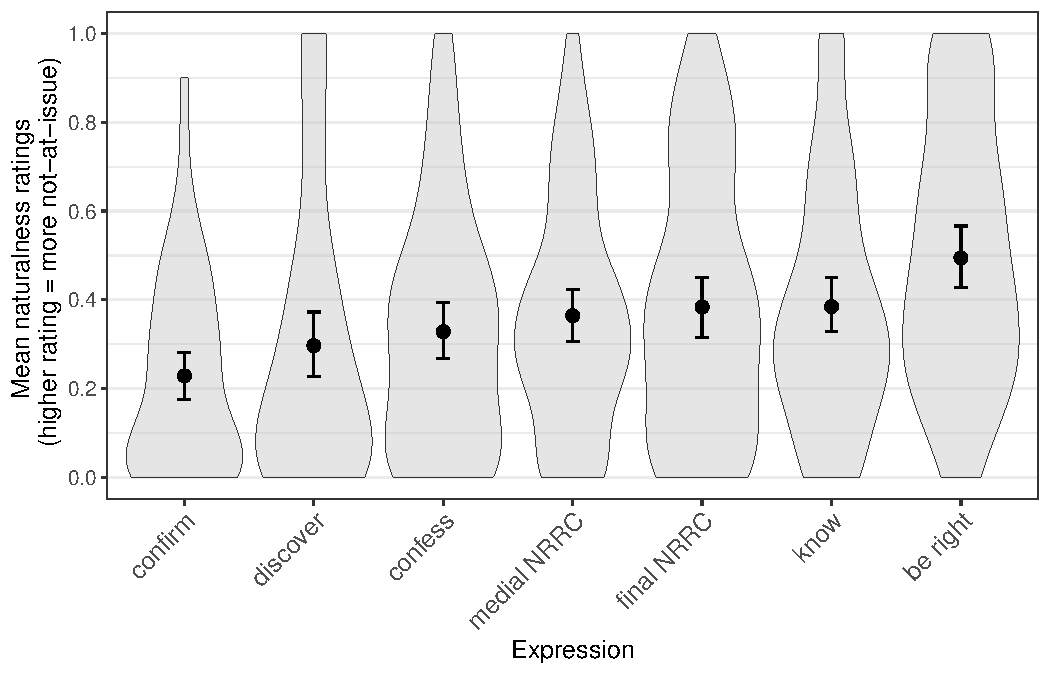
\includegraphics[width=1\textwidth]{../../results/main/exp1/graphs/mean-ratings.pdf}
 \caption{Exp.~1: QUD diagnostic}
 \end{subfigure} %
 \begin{subfigure}{.49\textwidth}
\centering
 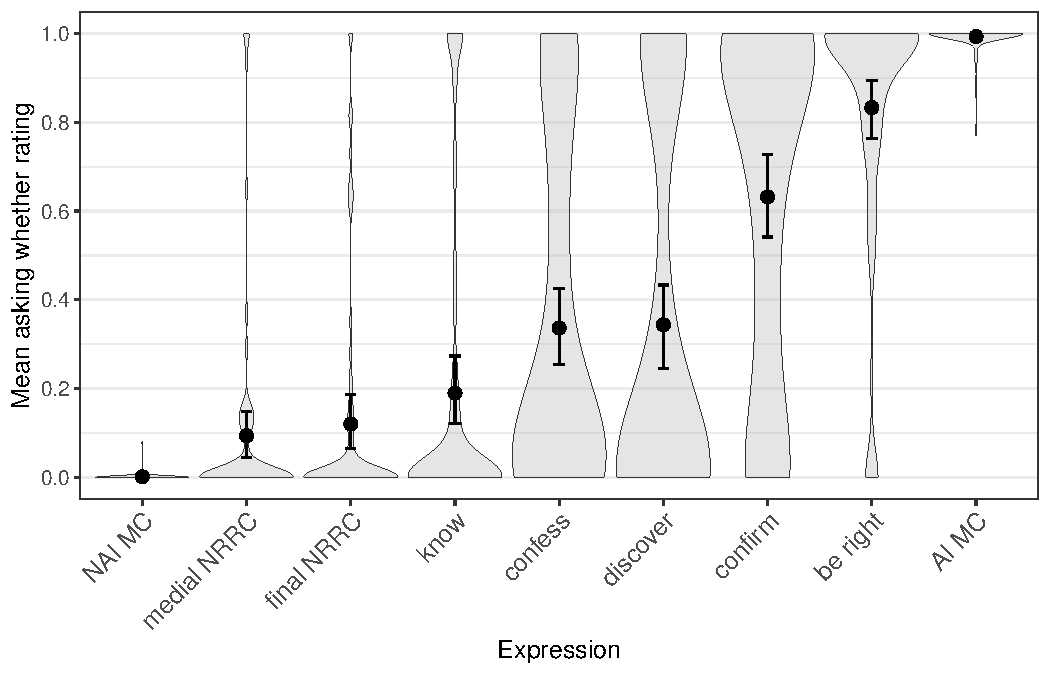
\includegraphics[width=1\textwidth]{../../results/main/exp2/graphs/mean-ratings.pdf}
 \caption{Exp.~2: `asking whether' diagnostic}
 \end{subfigure}


\begin{subfigure}{.49\textwidth}
\centering
 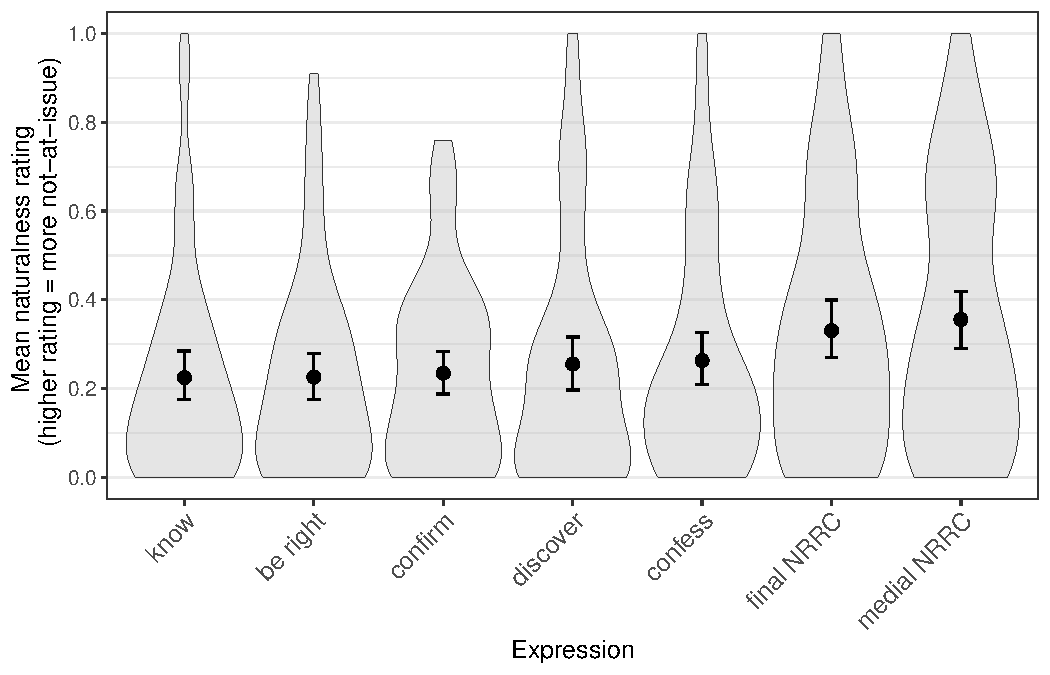
\includegraphics[width=1\textwidth]{../../results/main/exp3/graphs/mean-ratings.pdf}
 \caption{Exp.~3: `direct dissent' diagnostic}
 \end{subfigure} %
 \begin{subfigure}{.49\textwidth}
\centering
 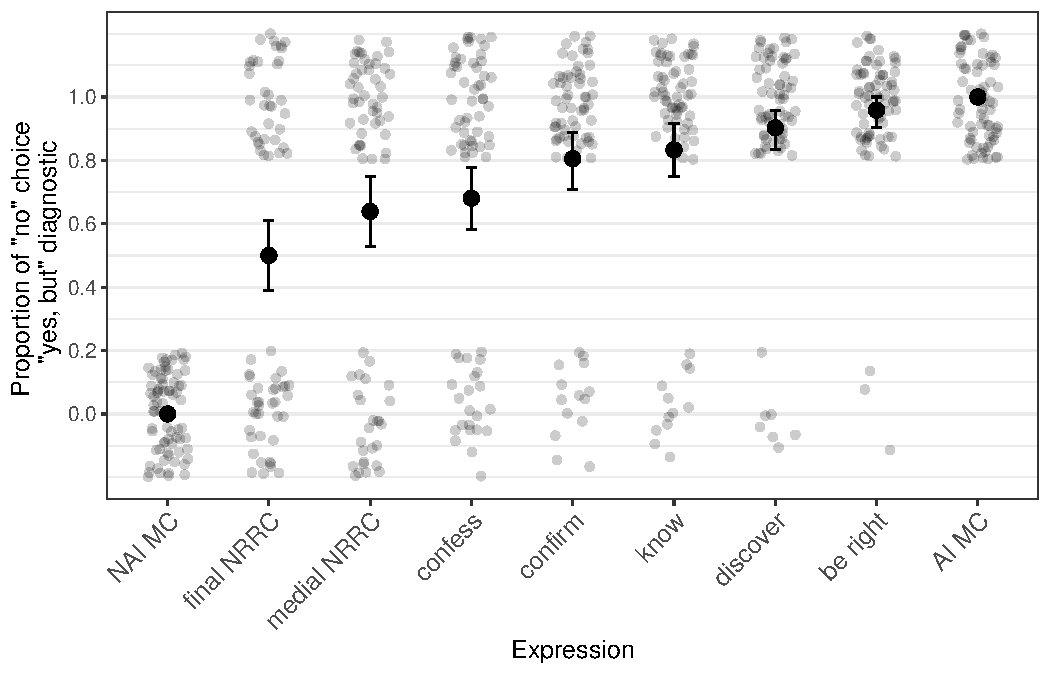
\includegraphics[width=1\textwidth]{../../results/main/exp4/graphs/mean-ratings.pdf}
 \caption{Exp.~4: `yes, but' diagnostic}
 \end{subfigure}

\caption{Results of Exps.~1-4. Panels (a)-(c) show the mean responses by content for the QUD-diagnostic in Exp.~1 (a), for the `asking whether' diagnostic in Exp.~2 (b), and for the `direct dissent' diagnostic in Exp.~3 (c). Panel (d) shows the proportion of `no' choices by content for the `yes, but' diagnostic in Exp.~4. Error bars indicate 95\% bootstrapped confidence intervals. Violin plots in panels (a)-(c) indicate the kernel probability density of the individual participants’ ratings. The gray dots in panel (d) individual participant responses (either ‘no’ or one of the ‘yes’-responses, jittered vertically and horizontally for legibility).} \label{fig:results}

\end{figure}

    % followed by \emph{confirm}, then \emph{confess}
%    \begin{figure}[ht]
%
%      \caption{Mean responses by content for the QUD-diagnostic (a), `asking whether' diagnostic (b), and `direct dissent' diagnostic (c). Error bars indicate 95\% bootstrapped confidence intervals. Violin plots indicate the kernel probability density of the individual participants’ ratings, which were given on a 0--1 scale, by adjusting a slider.} \label{fig:slider-ratings}
%
%      \centering
%      \subfloat[Answer match ratings for the QUD-diagnostic]{
%            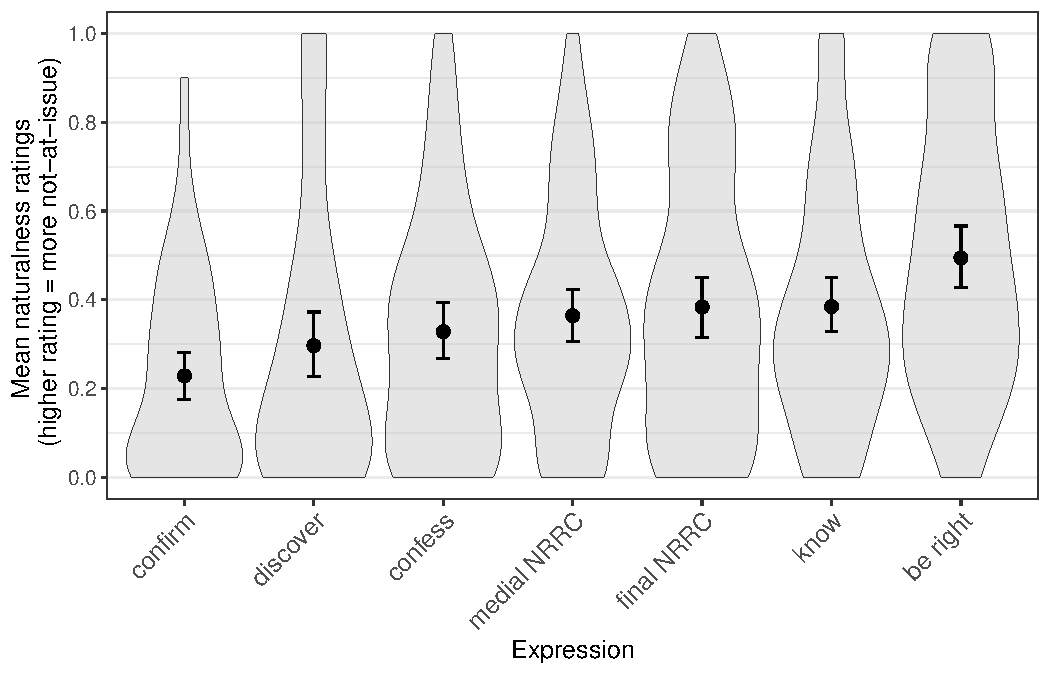
\includegraphics[width=.48\textwidth]{../../results/main/exp1/graphs/mean-ratings.pdf}
%            \label{fig:qud}
%        }
%        \subfloat[`asking whether' ratings]{
%            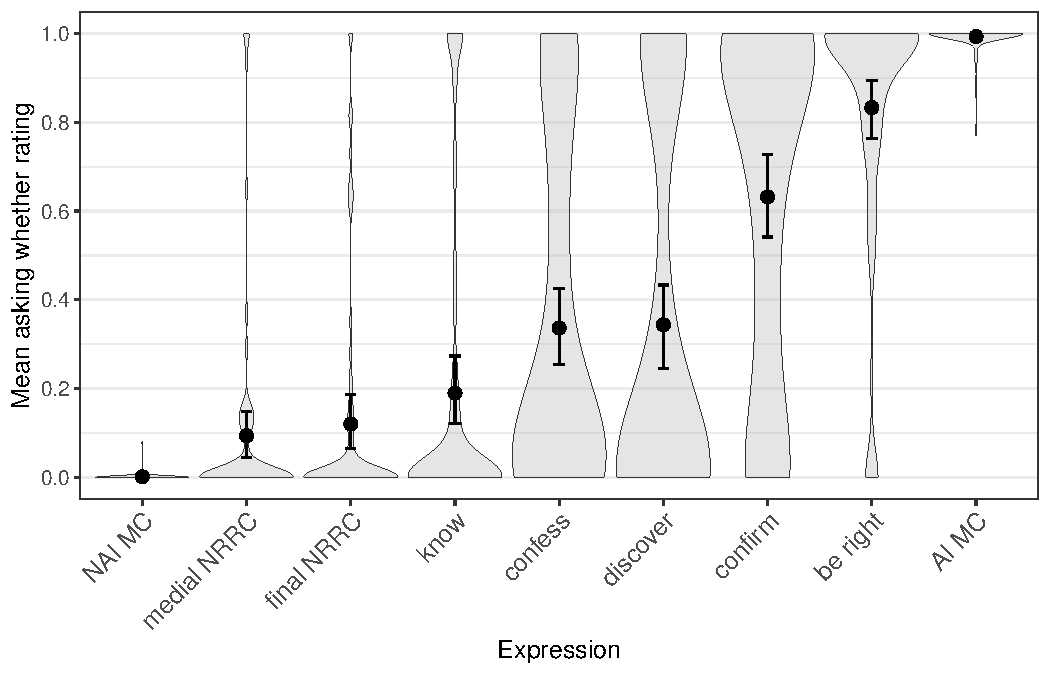
\includegraphics[width=.48\textwidth]{../../results/main/exp2/graphs/mean-ratings.pdf}
%            \label{fig:AK}
%        }\\
%        \vspace{-\baselineskip}
%        \subfloat[Naturalness ratings for the `direct dissent' diagnostic]{
%            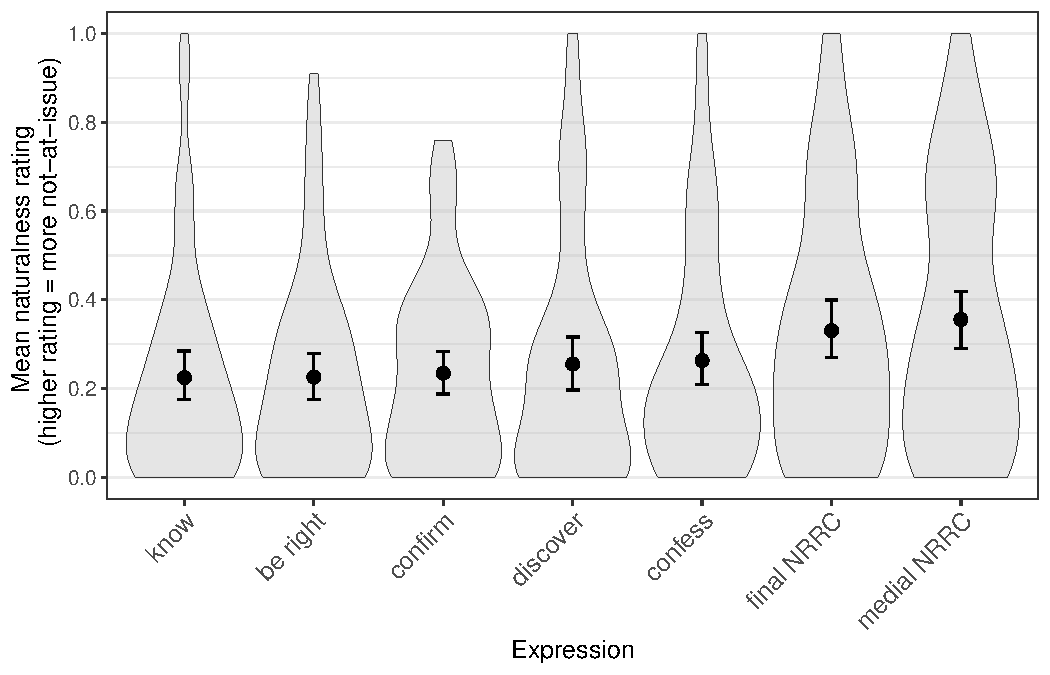
\includegraphics[width=.48\textwidth]{../../results/main/exp3/graphs/mean-ratings.pdf}
%            \label{fig:dd}
%        }
%    \end{figure}
%
%    \begin{figure}[ht]
%    \vspace{-2\baselineskip}
%      \caption{Proportion of ‘no’ choices by content for the `yes but' diagnostic. Error bars indicate 95\% bootstrapped confidence intervals. Gray dots indicate individual participant responses (either ‘no’ or one of the ‘yes’-responses, jittered vertically and horizontally for legibility).} \label{fig:yb}
%      \vspace{-.5\baselineskip}
%      \centering
%      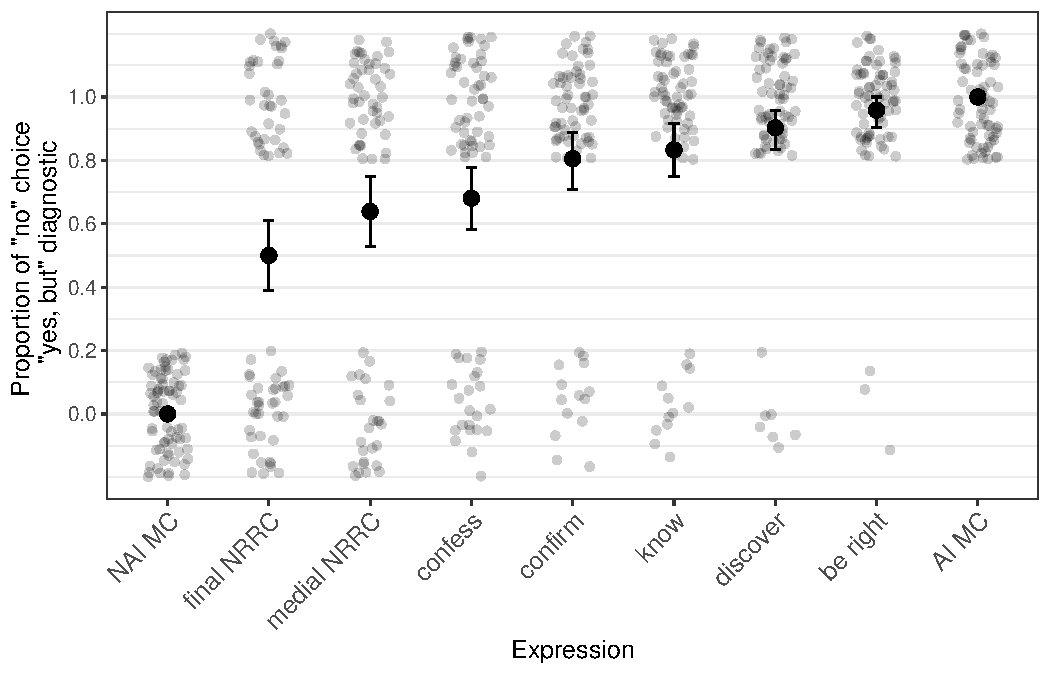
\includegraphics[width=.48\textwidth]{../../results/main/exp4/graphs/mean-ratings.pdf}
%    \end{figure}

    Second, the content manipulation affects the ratings differently across the four diagnostics, sometimes in opposite directions. This results in a different order of predicates by response means between experiments.
    \begin{itemize}
      \item For instance, \emph{be right} ranks highest under the `asking whether' diagnostic (\Cref{fig:AK}), and the `yes, but' test (\Cref{fig:yb}), but ranks lowest under the QUD-diagnostic (\Cref{fig:qud}), and shows no clear effect in the direct dissent diagnostic (\Cref{fig:dd}).
    \end{itemize}
    
    \begin{itemize}
      \item Analysis similar to what we did in projection study? -- Interaction effects
      \item How about something similar to the rank-analysis that Yvonne Kilian did for comparing diagnostics?

    \end{itemize}


  \subsection{Discussion}
    The differening results between diagnostics suggest that they are not interchangeable.

    \subsubsection{Sensitivity}

      \begin{itemize}
        \item Further, while the `asking whether' diagnostic, for contents embedded in questions, is sensitive enough to detect fine-grained differences between contents, the smaller range of response means for the other diagnostics could suggest the need for a more sensitive diagnostic for contents embedded in declarative assertions.

        \item We did not replicate the effect reported in \citealt{syrett_experimental_2015}, that sentence-final NRRCs receive higher at-issueness ratings than sentence-medial ones.

        \item  Additional comparison to \citealt{syrett_experimental_2015} (details omitted in the abstract) points to potential effects of the response task and the speech act of the utterance embedding the tested content.

      \end{itemize}

    \subsubsection{Order}

      \begin{itemize}
        \item In particular, the varying relative order of by-content means across diagnostics provide an initial argument that they target distinct properties of the content.
      \end{itemize}


\section{Conlusions and outlook}

  \subsection{Forward vs backward looking} % (fold)
    \begin{itemize}
      \item Q-AI ness + QUD diagnostic are about previous discourse
      \item P-AI ness and tonhauser's (\emph{issue} I-AI ness) are about the upcoming discourse
      \item can utterances shift the QUD? QUD-stack; adèle hernot-mortier?
      \item conditionals, sentence-medial vs sentence-final appositives
      \item co-ordination vs subordinating discourse relations and moving the discourse forward 
      \item possible confound: do the direct dissent diagnostic and the `yes, but' test P-at-issueness or anaphoric availability (\cite{snider_distinguishing_2018})
    \end{itemize}  
  
  % subsection forward_vs_backward_looking (end)

  \subsection{Questions vs assertions} % (fold)
      \begin{itemize}
        \item Q-AI ness and I-AIness are about question partitions
        \item P-AI ness is about assertive proposals
        \item is the speech-act distinction relevant? table model (and potentially some QUD implementations) suggest that this difference shouldnt matter
        \item possible counfound: commitment related to projection that we discussed in relation to the big study
      \end{itemize}
      
      \paragraph{Based on our data:} % (fold)
      
      \begin{itemize}
        \item the speech act seems to matter: the `asking whether' diagnostic, targeting questions...
      \end{itemize}

  % subsection questions_and_assertions (end)

  \subsection{Other diagnostics} % (fold)
    
  
  % subsection other_diagnostics (end)

  \begin{itemize}
    \item Other diagnostics (Horn on argumentation / because-clauses; evaluative adjectives)
  \end{itemize}


\pagebreak
\bibliographystyle{plainnat}
\bibliography{../at-issueness}

  

\end{document}